\documentclass[11 pt, a4paper]{article}


\NeedsTeXFormat{LaTeX2e}
\usepackage{layout}
\usepackage{setspace} %augmenter localement interligne

% Extensions
\RequirePackage{geometry} 
\geometry{a4paper,tmargin=1.2cm,bmargin=0.8cm,lmargin=1.5cm,rmargin=0.5cm}

% Paramètres du titre
% *******************
\def\classe{$1^{\text{re}}$-Spécialité mathématiques}
\def\titre{Chapitre 1 : Équations, fonctions polynômes du second degré}
\def\site{}

\title{\titre}
%\date{~-07-09-12-}
\date{}
\author{\classe}



% Debut du document
% *****************

\begin{document}
\renewcommand{\labelitemi}{$\star$}
\maketitle

% Debut du texte
% **************

\normalsize


\section{Fonctions polynôme de degré 2}
	\subsection{Les fonctions $x \mapsto ax^2+bx+c$ avec $a \neq 0$}
\begin{Df} ~\\	
Une \textbf{fonction polynôme de degré 2} est une fonction définie sur $\R$ par $f(x)=ax^2+bx+c$ où $a$, $b$ et $c$ désignent des nombres réels avec $a\neq 0$. Cette écriture est la \textbf{forme développée} de $f$.
\end{Df}	

%\Rq{~ \\
%L'expression $ax^2+bx+c$ avec $a\neq 0$ est aussi appelée \textbf{trinôme du second degré} ou plus simplement \textbf{trinôme}.
%}


\Rq{
Une fonction polynôme du second degré est aussi appelée fonction trinôme du second degré ou plus simplement fonction trinôme.
}


	\subsection{Forme canonique}
\Prp{
Toute fonction polynôme de degré 2 définie par $f(x)=ax^2+bx+c$ avec $a\neq 0$ admet pour \textbf{forme canonique} $f(x)=a(x-\alpha)^2+\beta$ avec $\alpha=-\dfrac{b}{2a}$ et $\beta = f(\alpha)$. 
}

\begin{Dm}~ \\
Soit $f$ une fonction polynôme de degré 2 définie par $f(x)=ax^2+bx+c$.\\
Posons $\alpha=-\dfrac{b}{2a}$ et $\beta = f(\alpha)$.\\
Alors, pour tout nombre réel $x$ : 
\begin{spacing}{1.7}
	$a(x-\alpha)^2+\beta=$ \dotfill \\.\dotfill \\.\dotfill \\.\dotfill \\.\dotfill\\ .\dotfill \\ .\dotfill \\ .\dotfill
\end{spacing}
\end{Dm}

%\vspace{0.5cm}
\begin{Ex}
Déterminer la forme canonique de la fonction trinôme définie sur $\R$ par $f(x)=-4x^2+6x+\dfrac{5}{4}$.
\begin{spacing}{1.7}
 .\dotfill \\ .\dotfill \\ .\dotfill \\ .\dotfill \\ .\dotfill \\ .\dotfill \\ .\dotfill \\ .\dotfill
\end{spacing}
\end{Ex}

\newpage
\begin{Rq}
	\begin{spacing}{1.5}
	Dans l'exemple précédent, la plus grande valeur possible (\textbf{le maximum})de $f(x)$ est ............ et cette valeur est atteinte lorsque $x = ...............$ .
	\end{spacing}
\end{Rq}

	\subsection{Courbe représentative et variations}

\vspace{-0.8cm}

\Prp{
\small{
\phantom{es}
\I Dans un repère orthogonal du plan, $f$ est représentée par une parabole $\mathcal P$ dont le sommet $S(\alpha ; \beta)$  et l'axe de symétrie a pour équation $x=\alpha$.


\begin{tabularx}{\linewidth}{>{\centering \arraybackslash}X|>{\centering \arraybackslash}X}
\rule[-2ex]{0pt}{6ex}
\fbox{cas $a>0$}&\fbox{cas $a<0$}\\ 
La parabole est \og tournée vers le haut\fg & La parabole est \og tournée vers le bas\fg \\
\psset{unit=.5cm}
\begin{pspicture}(-8,-5)(4,6)
\def\pshlabel#1{\footnotesize #1}
\def\psvlabel#1{\footnotesize #1}
\def\f{.25*x^2+x-3}
\newrgbcolor{bleu}{0.1 0.05 .5}
\newrgbcolor{prune}{.6 0 .48}
\psaxes[labelsep=.8mm,linewidth=.75pt,ticks=none, labels=none]{->}(0,0)(-8,-5)(4,6)
\psaxes[labels=none,linewidth=1pt,linecolor=prune,ticks=none]{->}(0,0)(1.2,1.2)
\uput[dl](0,0){\footnotesize{O}}
\uput[d](.6,0){\prune{\footnotesize{$\vec{i}$}}}\uput[l](0,0.6){\prune{\footnotesize{$\vec{j}$}}}
\uput[dl](4,0){\footnotesize{$x$}} \uput[dl](0,6){\footnotesize{$y$}}
\psplot[algebraic=true,plotpoints=500,linewidth=1.25pt, linecolor=bleu]{-8}{4}{\f}
\psline[linewidth=.5pt,linestyle=dashed,linecolor=prune](-2,-5)(-2,6)
\psline[linewidth=.5pt,linestyle=dashed,linecolor=prune](0,-4)(-2,-4)
\uput[dl](-2,-4){\prune{\footnotesize{$S$}}}
\uput[r](0,-4){\prune{\footnotesize{$f\left(-\dfrac{b}{2a}\right)$}}}
\uput[dl](-2,0){\prune{\footnotesize{$-\dfrac{b}{2a}$}}}
\end{pspicture}
&
\psset{unit=.5cm}
\begin{pspicture}(-4,-5)(8,6)
\def\pshlabel#1{\footnotesize #1}
\def\psvlabel#1{\footnotesize #1}
\def\f{-.25*x^2+x+3}
\newrgbcolor{bleu}{0.1 0.05 .5}
\newrgbcolor{prune}{.6 0 .48}
\psaxes[labelsep=.8mm,linewidth=.75pt,ticks=none, labels=none]{->}(0,0)(-4,-5)(8,6)
\psaxes[labels=none,linewidth=1pt,linecolor=prune,ticks=none]{->}(0,0)(1.2,1.2)
\uput[dl](0,0){\footnotesize{O}}
\uput[d](.6,0){\prune{\footnotesize{$\vec{i}$}}}\uput[l](0,0.6){\prune{\footnotesize{$\vec{j}$}}}
\uput[dl](8,0){\footnotesize{$x$}} \uput[dl](0,6){\footnotesize{$y$}}
\psplot[algebraic=true,plotpoints=500,linewidth=1.25pt, linecolor=bleu]{-4}{8}{\f}
\psline[linewidth=.5pt,linestyle=dashed,linecolor=prune](2,-5)(2,6)
\psline[linewidth=.5pt,linestyle=dashed,linecolor=prune](0,4)(2,4)
\uput[ur](2,4){\prune{\footnotesize{$S$}}}
\uput[l](0,4){\prune{\footnotesize{$f\left(-\dfrac{b}{2a}\right)$}}}
\uput[dr](2,0){\prune{\footnotesize{$-\dfrac{b}{2a}$}}}
\end{pspicture}\\
%\end{tabularx}
%\medskip
%\begin{tabularx}{\linewidth}{>{\centering \arraybackslash}X|>{\centering \arraybackslash}X}
%\rule[-2ex]{0pt}{6ex}
%\fbox{cas $a<0$}&\fbox{cas $a>0$}\\ 
\\
\begin{tikzpicture}
\tkzTabInit[lgt=2,espcl=2.7]{$x$/0.9, Variations de $f$/2.4}{$-\infty$ ,$-\dfrac{b}{2a}$,$+\infty$}
%\tkzTabLine{,-,z,+,}
\tkzTabVar{+/,-/\small{ $f(-\dfrac{b}{2a})$},+/}
%\valeur[draw,]{2}{4}{1}
%\tkzTabVal{1}{3}{0.5}{}{$1$}
\end{tikzpicture} 
&
\begin{tikzpicture}
\tkzTabInit[lgt=2,espcl=2.7]{$x$/0.9, Variations de $f$/2.4}{$-\infty$ ,$-\dfrac{b}{2a}$,$+\infty$}
%\tkzTabLine{,-,z,+,}
\tkzTabVar{-/,+/\small{ $f(-\dfrac{b}{2a})$},-/}
%\valeur[draw,]{2}{4}{1}
%\tkzTabVal{1}{3}{0.5}{}{$1$}
\end{tikzpicture} 
\end{tabularx}
}
}

\begin{Rq} ~\\
	Dans le cas où $a > 0$, $f$ admet donc un ........................... qui vaut ................................... et qui est atteint lorsque $x =$ ................\\ ~\\
	Dans le cas où $a < 0$, $f$ admet donc un ........................... qui vaut ................................... et qui est atteint lorsque $x =$ ................
\end{Rq}

\begin{Ex}
	Soit $f$ la fonction du second degré de forme canonique $f(x)=-3\left( x + 2\right)^{2} - 1$.\\
	Dessiner l'allure de la courbe de $f$ dans un repère puis dresser son tableau de variation. 
\end{Ex}

\newpage


\section{Équations du second degré}
Soit $f$ une fonction polynôme du second degré définie sur $\R$ par $f(x)=ax^2+bx+c$.\\
On apprend ici à résoudre l'équation $f(x)=0$ soit $ax^2+bx+c=0$. 
	\subsection{Définitions}

\begin{Df} ~\\	
Une \textbf{équation du second degré} à coefficients réels est une équation de la forme $ax^2+bx+c=0$, avec $a$, $b$ et $c$ trois réels tels que $a\neq 0$.
\end{Df}	

\begin{Df} ~\\	
Les solutions de l'équation du second degré $ax^2+bx+c=0$ sont appelées les \textbf{racines} du polynôme du second degré $ax^2+bx+c$.
\end{Df}	


	\subsection{Résolution d'une équation du second degré dans $\R$}

\begin{Df} ~\\	
Le nombre réel $b^2-4ac$ est appelé \textbf{discriminant} du trinôme $ax^2+bx+c$. Il est noté $\Delta$.
\end{Df}

\Thm{
Résolution de l'équation $ax^2+bx+c=0$ avec $a\neq 0$.\\
On calcule le discriminant : $\Delta= b^2-4ac$.
\begin{itemize}
\item[$\bullet$] Si $\Delta < 0 $ : l'équation n'admet pas de solution réelle;
\medskip
\item[$\bullet$] Si $\Delta = 0 $ : L'équation admet une unique solution réelle $x_0=-\dfrac{b}{2a}$ ;
\medskip
\item[$\bullet$] Si $\Delta > 0 $ : L'équation admet deux solutions réelles distinctes $x_1=\dfrac{-b-\sqrt{\Delta}}{2a}$ et $x_2=\dfrac{-b+\sqrt{\Delta}}{2a}$.
\end{itemize}
}


\begin{DmI} Voir activité 
%Montrer que résoudre l'équation $ax^2+bx+c=0$ ($a\neq 0$) revient à résoudre $\left(x+\dfrac{b}{2a}\right)^2-\dfrac{\Delta}{4a^2}=0$.% (factorisation canonique).
%
%\vspace{2.5cm}
%
%
%\I Le nombre de solutions dépend du signe de $\Delta$.
%
%\begin{itemize}
%\item[$\bullet$] 
%\medskip
%\medskip
%\medskip
%\medskip
%\item[$\bullet$]  
%\medskip
%\medskip
%\medskip
%\medskip
%\medskip
%\item[$\bullet$] 
%\medskip
%\medskip
%\medskip
%\medskip
%\medskip
%\end{itemize}
\end{DmI}

\bigskip


\begin{Ex}\label{ex1}
Résoudre dans $\R$ les équations suivantes : %(utiliser les résultats de l'\textbf{exemple \ref{ex}}) :
\vspace{-0.4cm}
\begin{tabenum} %\qquad %\qquad
\item $-x^2-4x+21=0$\qquad \qquad \qquad
\item $3x^2 -x+1=0$\qquad \qquad \qquad
\item $4x^2+6x+\dfrac{9}{4}=0$
\end{tabenum}
\end{Ex}

\vspace{5cm}

%\begin{Ex}
%Pierre affirme : \og L'équation $-x^2-2x-2=0$ a deux solutions \fg{}. Que peut-on en penser ? 
%\end{Ex}


\newpage



	\subsection{Interprétation graphique}
	
\vspace{-0.7cm}

\Prp{
\begin{tabular}{|c|c|c|c|}
\hline 
\phantom{$\dfrac{A}{A}$} Signe de $\Delta$ & $\Delta>0$ & $\Delta =0$ & $\Delta < 0 $ \\ 
\hline 
\phantom{$\dfrac{A}{A}$} Solution de l'équation  & Deux solutions réelles distinctes& Une unique solution &  \\ 
$ax^2+bx+c=0$ & $x_1=\dfrac{-b-\sqrt{\Delta}}{2a}$ et $x_2=\dfrac{-b+\sqrt{\Delta}}{2a}$& $x_0=-\dfrac{b}{2a}$ & Pas de solution réelle \\ 
 & &  & \\ 
\hline 
Courbe représentative & &  & \\ 
de $f$ dans un repère & &  & \\ 
\danger Dans le cas où $a>0$  & 
\centering
\def\xmin{-2.6} \def\xmax{2.6} \def\ymin{-3.1} \def\ymax{2.6}
\psset{xunit=0.75cm,yunit=0.75cm}
\begin{pspicture*}(\xmin,\ymin)(\xmax,\ymax)
\psaxes[labels=none,labelsep=1pt, Dx=10,Dy=10]{->}(0,0)(\xmin,\ymin)(\xmax,\ymax)
\uput[dl](0,0){$O$}
\uput[dl](\xmax,0){$x$}
\uput[dr](0,\ymax){$y$}
\psplot[plotpoints=200,algebraic=true]{\xmin}{\xmax}{(x-1)*(x+2)}
\psline[linestyle=dashed](-0.5,0)(-0.5,-2.25)
\uput[u](-0.5,0){\footnotesize $-\frac{b}{2a}$}
\psdots[dotstyle=x](1,0)(-2,0)
\uput[ur](-2,0){$x_1$}
\uput[ul](1,0){$x_2$}
\end{pspicture*}
 & \centering
\def\xmin{-2.0} \def\xmax{2.6} \def\ymin{-1.1} \def\ymax{4.6}
\psset{xunit=0.6cm,yunit=0.6cm}
\begin{pspicture*}(\xmin,\ymin)(\xmax,\ymax)
\psaxes[labels=none,labelsep=1pt, Dx=10,Dy=10]{->}(0,0)(\xmin,\ymin)(\xmax,\ymax)
\uput[dl](0,0){$O$}
\uput[dl](\xmax,0){$x$}
\uput[dr](0,\ymax){$y$}
\psplot[plotpoints=200,algebraic=true]{\xmin}{\xmax}{(x-1)^2}
%\psline[linestyle=dashed](-1,0)(-1,1)
\psdot[dotstyle=x](1,0)
\uput[d](1,0){\footnotesize $x_0=-\frac{b}{2a}$}
\end{pspicture*}
 & \centering
\def\xmin{-2.6} \def\xmax{2.0} \def\ymin{-1.1} \def\ymax{4.6}
\psset{xunit=0.6cm,yunit=0.6cm}
\begin{pspicture*}(\xmin,\ymin)(\xmax,\ymax)
\psaxes[labels=none,labelsep=1pt, Dx=10,Dy=10]{->}(0,0)(\xmin,\ymin)(\xmax,\ymax)
\uput[dl](0,0){$O$}
\uput[dl](\xmax,0){$x$}
\uput[dr](0,\ymax){$y$}
\psplot[plotpoints=200,algebraic=true]{\xmin}{\xmax}{(x+1)^2+1}
\psline[linestyle=dashed](-1,0)(-1,1)
\uput[d](-1,0){\footnotesize $-\frac{b}{2a}$}
\end{pspicture*}
 \tabularnewline \\ 
\hline 
\end{tabular} 
}

	
\Rq{ ~
\begin{itemize}
\item Chercher à résoudre l'équation $ax^2+bx+c=0$ revient à chercher les points d'intersection de la parabole $\mathcal P :ax^2+bx+c $ avec l'axe des abscisses.
%\item Les solutions de l'équation $ax^2+bx+c=0$ sont aussi appelées \textbf{racines} du trinôme.
\item Dans le cas où $\Delta =0$, l'unique solution $x_0$ est appelée racine double du trinôme (dans ce cas $x_1=x_2$).
\end{itemize}
}



%\section{Somme est produit d'une fonction polynôme du second degré}
%\section{Somme et produit des racines d'un trinôme}
\subsection{Somme et produit des racines d'un trinôme}

\Prp{
Soit $f$ une fonction polynôme du second degré définie sur $\R$ par $f(x)=ax^2+bx+c$, avec $a\neq 0$.\\
Si $f$ admet les réels $x_1$ et $x_2$ pour racines, alors :
\begin{itemize}
\item[$\bullet$] La \textbf{somme} des racines est : $s=x_1+x_2=-\dfrac{b}{a}$;
\medskip
\item[$\bullet$] Le \textbf{produit} des racines est : $p=x_1 \times x_2=\dfrac{c}{a}$.
\end{itemize}
}

\Rq{ ~
Si on connaît une racine d'une fonction polynôme du second degré, on peut calculer l'autre racine en utilisant la somme ou le produit des racines. \\
Lorsque cela est possible, on cherchera une \textbf{racine évidente} parmi des nombres simples comme $1$, $-1$, $2$, $-2$, etc.
}



\begin{Dm}~\\
\end{Dm}

\bigskip
\bigskip
\bigskip
\bigskip
\bigskip

\begin{Ex}
Soit $f$ la fonction définie sur $\R$ par $f(x)=-2x^2+3x+2$. Déterminer une racine évidente de $f$, puis l'autre solution.
\end{Ex}

\bigskip
\bigskip

%\Prp{
%Deux nombres réels ont pour somme $s$ et pour produit $p$ si, et seulement si, ils sont racines de la fonction polynôme du second degré $x \mapsto x^2-sx+p$. 
%}
%
%\begin{Dm}~\\
%Démontrer que les réels $x_1$ et $x_2$ tels que $s=x_1+x_2$ et $p=x_1 \times x_2$ sont solutions de l'équation $x^2-sx+p=0$.
%\end{Dm}
%
%
%\bigskip
%\bigskip


\begin{Ex}
Déterminer une fonction polynôme du second degré admettant les racines $-6$ et $8$.
\end{Ex}


\newpage

\section{Factorisation et signe d'un trinôme du second degré}
%$f$ est ne fonction polynôme de degré 2 est une fonction définie sur $\R$ par $f(x)=ax^2+bx+c$  avec $a\neq 0$.\\
%Son discriminant est $\Delta= b^2-4ac$
%\I Soit le trinôme $ax^2+bx+c$ avec $a\neq 0$ et $\Delta$ son discriminant.

	\subsection{Forme factorisée d'un trinôme de degré 2}
\Prp{
Soit le trinôme $ax^2+bx+c$ avec $a\neq 0$ et $\Delta$ son discriminant.
%Selon les valeurs du discriminant $\Delta$, on peut factoriser la fonction $f$ %polynôme de degré 2
\begin{itemize}
\item[$\bullet$] Si $\Delta > 0$, alors pour tout réel $x$, $ax^2+bx+c=a(x-x_1)(x-x_2)$ où $x_1$ et $x_2$ sont les racines du trinôme.
\item[$\bullet$] Si $\Delta = 0$, alors pour tout réel $x$, $ax^2+bx+c=a(x-x_0)^2$ où $x_0$ est la racine double du trinôme.
\item[$\bullet$] Si $\Delta < 0$, le trinôme ne se factorise pas.
\end{itemize}
}	


\begin{Ex}\label{ex2}
Factoriser les trinômes suivants (utiliser les résultats de l'\textbf{exemple \ref{ex1}}) :
%\vspace{-0.4cm}
\bigskip
\begin{enumerate}
 %\qquad %\qquad
\item $-5x^2+8x-2$\qquad \qquad \qquad \qquad
\bigskip
\item $3x^2 -x+1$\qquad \qquad \qquad \qquad
\bigskip
\item $4x^2+6x+\dfrac{9}{4}$
\end{enumerate}
\end{Ex}

%\vspace{2.5cm}


	\subsection{Signe du trinôme $ax^2+bx+c$ avec $a\neq 0$}
	
\Prp{
Soit le trinôme $ax^2+bx+c$ avec $a\neq 0$ et $\Delta$ son discriminant.
\begin{itemize}
\item[$\bullet$] Si $\Delta > 0$, le trinôme s'annule en deux réels distincts $x_1$ et $x_2$.\\
Si $x_1 <x_2$, le tableau de signes du trinôme est :

\begin{tikzpicture}
\tkzTabInit[lgt=4.5,espcl=3] {$x$/0.8,Signe de $ax^2+bx+c$ /0.8}{$-\infty$,$x_1$, $x_2$ , $+\infty$}
\tkzTabLine{,$signe de $ a,z,$signe de $-a,z,$signe de $ a,}
%\tkzTabVar{-/$0$, R/,+/$+\infty$}
%\valeur[draw,]{}{4}{1}{}{0}
%\tkzTabVal{1}{3}{0.5}{}{$1$}
\end{tikzpicture}

\item[$\bullet$] Si $\Delta = 0$, le trinôme a même signe que $a$ pour tout réel $x$ et s'annule en $-\dfrac{b}{2a}$.
\item[$\bullet$] Si $\Delta < 0$, le trinôme a même signe que $a$ pour tout réel $x$.
\end{itemize}
}	
	
\begin{Ex}
Déterminer le signe des trinômes suivants (utiliser, si besoin, les résultats de l'\textbf{exemple \ref{ex1}}) :
\begin{enumerate}
 %\qquad %\qquad
\item $-5x^2+8x-2$\qquad \qquad \qquad \qquad
\bigskip
\bigskip
\bigskip
\bigskip
\bigskip
\item $3x^2 -x+1$\qquad \qquad \qquad \qquad
\bigskip
\bigskip
\bigskip
\bigskip
\bigskip
\item $4x^2+6x+\dfrac{9}{4}$
\bigskip
\end{enumerate}
\end{Ex}

\bigskip
\bigskip
%\vspace{4cm}

\begin{Ex}
Paul affirme : \og L'inéquation $x^2+4x-4<0$ n'a pas de solution \fg{}. Que peut-on en penser ? 
\end{Ex}




\renewcommand{\fin}{{\scriptsize \site}\hfil {\scriptsize  \titre}\hfil \upshape {\thepage\slash \pageref{LastPage}}}


\end{document}


